% \iffalse
\let\negmedspace\undefined
\let\negthickspace\undefined
\documentclass[journal,12pt,twocolumn]{IEEEtran}
\usepackage{cite}
\usepackage{amsmath,amssymb,amsfonts,amsthm}
\usepackage{algorithmic}
\usepackage{graphicx}
\usepackage{textcomp}
\usepackage{xcolor}
\usepackage{txfonts}
\usepackage{listings}
\usepackage{enumitem}
\usepackage{mathtools}
\usepackage{gensymb}
\usepackage{comment}
\usepackage[breaklinks=true]{hyperref}
\usepackage{tkz-euclide} 
\usepackage{listings}
\usepackage{gvv}                                        
\def\inputGnumericTable{}                                 
\usepackage[latin1]{inputenc}                                
\usepackage{color}                                            
\usepackage{array}                                            
\usepackage{longtable}                                       
\usepackage{calc}                                             
\usepackage{multirow}                                         
\usepackage{hhline}                                           
\usepackage{ifthen}                                           
\usepackage{lscape}
\newtheorem{theorem}{Theorem}[section]
\newtheorem{problem}{Problem}
\newtheorem{proposition}{Proposition}[section]
\newtheorem{lemma}{Lemma}[section]
\newtheorem{corollary}[theorem]{Corollary}
\newtheorem{example}{Example}[section]
\newtheorem{definition}[problem]{Definition}
\newcommand{\BEQA}{\begin{eqnarray}}
\newcommand{\EEQA}{\end{eqnarray}}
\newcommand{\define}{\stackrel{\triangle}{=}}
\theoremstyle{remark}
\newtheorem{rem}{Remark}
\begin{document}

\bibliographystyle{IEEEtran}
\vspace{3cm}

\title{10.5.3.9}
\author{EE23BTECH11063 - Vemula Siddhartha
}
\maketitle
\newpage
\bigskip

\renewcommand{\thefigure}{\theenumi}
\renewcommand{\thetable}{\theenumi}
\textbf{Question}:\\
If the sum of first 7 terms of an AP is 49 and that of 17 terms is 289, find the sum of
first n terms.
\\\\
\textbf{Solution: }
\begin{align}
S\brak{n}&=\frac{n}{2}\,\brak{2x\brak{0}+\brak{n-1}\,d}\label{eq10.5.3.9.1}\\
S\brak{7}&=49 \\
49&=\frac{7}{2}\,\brak{2x\brak{0}+\brak{7-1}\,d}  \\
49&=\frac{7}{2}\,\brak{2x\brak{0}+6d}  \\
x\brak{0}+3d&=7\label{eq10.5.3.9.2}\\
S\brak{17}&=289  \\
289&=\frac{17}{2}\,\brak{2x\brak{0}+\brak{17-1}\,d}  \\
289&=\frac{17}{2}\,\brak{2x\brak{0}+16d}  \\
x\brak{0}+8d&=17 \label{eq10.5.3.9.3}
\end{align}
From  equations \ref{eq10.5.3.9.2} and \ref{eq10.5.3.9.3}, the augmented matrix is:
\begin{align}\vspace{3cm}
 \begin{pmatrix}
1&3&7\\
1&8&17
 \end{pmatrix}
 \\
 R_2\rightarrow R_2-R_1\notag\\
 \begin{pmatrix}
    1&3&7\\
    0&5&10
 \end{pmatrix}
 \\
 R_1\rightarrow 5R_1-3R_2\notag\\
 \begin{pmatrix}
    5&0&5\\
    0&5&10
 \end{pmatrix}
 \\
 R_1\rightarrow\frac{1}{5}R_1\notag\\ R_2\rightarrow\frac{1}{5}R_2\notag\\
 \begin{pmatrix}
    1&0&1\\
    0&1&2
 \end{pmatrix}\\
 \implies
 \begin{pmatrix}
    x\brak{0}\\
    d
 \end{pmatrix}
 =
 \begin{pmatrix}
    1\\2
 \end{pmatrix}
\end{align}
\begin{align}
    \implies S\brak{n}&= \frac{n}{2}\,\brak{2x\brak{0}+\brak{n-1}\,d}\label{eq10.5.3.9.4}\\
    S\brak{n}&=n^2\label{eq10.5.3.9.5}
\end{align}
\begin{align}
    x\brak{n}&=\brak{x\brak{0}+nd}u\brak{n}\\
    \text{From \tabref{tab10.5.3.9.1}:}\notag\\
    \implies x\brak{n}&= \brak{1+2n}u\brak{n}\\
    &x\brak{n}\system{Z}X\brak{z}\notag\\
    X\brak{z}&=\frac{x\brak{0}}{1-z^{-1}}+\frac{dz^{-1}}{\brak{1-z^{-1}}^2}\\
    \text{From \tabref{tab10.5.3.9.1}:}\notag\\
    \implies X\brak{z}&=\frac{1+z^{-1}}{\brak{1-z^{-1}}^2} \;\;\cbrak{z\in\mathbb{C}: |z|>1}
\end{align}
\begin{figure}[h]
    \centering
    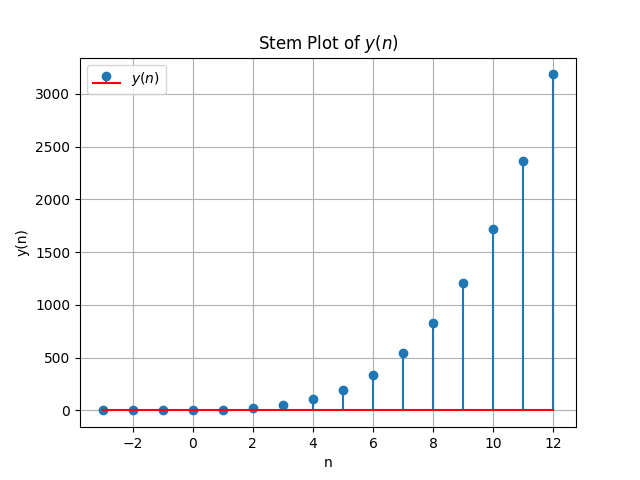
\includegraphics[width=1.1\linewidth]{Figure_1.png}
    \caption{Stem Plot of x\brak{n}}
    \label{stemplot}
\end{figure}
 \begin{table}[h]
    \centering
    \begin{tabular}[12pt]{ |c| c| c|}
    \hline
    \textbf{Variable} & \textbf{Description} &\textbf{Value}\\ 
    \hline
    $x\brak{0}$ & First term of the AP &1\\
    \hline 
    $d$ & Common difference of the AP& 2\\
    \hline
    $S\brak{n}$ & Sum of $n$ terms of the AP& $n^2$\\
    \hline
    $S\brak{7}$& Sum of 7 terms of the AP& 49\\
    \hline
    $S\brak{17}$& Sum of 17 terms of the AP&289\\
    \hline
    $x(n)$ & General term& $\brak{1+2n}\,u\brak{n}$\\
    \hline
    $X(z)$ & Z- transform of $x(n)$& $\frac{1+z^{-1}}{\brak{1-z^{-1}}^2} \cbrak{z\in\mathbb{C}: |z|>1}$\\
    \hline    
    \end{tabular}
    \caption{Variables Used}
    \label{tab10.5.3.9.1}
\end{table}
\end{document}  